% -*- coding: utf-8 -*-
% !TEX root = ../main.tex

% TODO Développer dans plusieurs sous-sections ce que vous avez réalisé pendant votre stage

\subsection{Organisation du repo pallas-analysis}\label{ssec:pallas_analysis_repo}

Le code ainsi que les graphiques réalisés lors de ce stage sont accessibles via le dépôt GitHub pallas-analysis \cite{pallas-analysis}.\newline
Ce dépôt regroupe les scripts \verb!bash! permettant d'installer et compiler \verb!PALLAS! avec \verb!EZTrace! ainsi que \verb!ZFP!, et des scripts 
\verb!python! permettant de réaliser les graphiques à partir des benchmarks lancés via des scripts \verb!bash!.
\newline
Ce dernier s'organise de la manière suivante :

\begin{figure}[!h]
\centering
\begin{minipage}{7cm}
\dirtree{%
.1 /pallas-analysis/.
    .2 analysis/.
        .3 prog/.
        .3 plot/.
        .3 results/.
    .2 build\_pallas\_eztrace/.
        .3 building\_eztrace\_pallas.sh.
        .3 setup\_all.sh.
    .2 run\_benchmarks/.
        .3 run\_nas\_benchmark/.
        .3 run\_lulesh/.
        .3 patches\_nas/.
        .3 divers scripts bash \( \ldots \).
    .2 Makefile.
    .2 README.md.
}
\end{minipage}
\caption{Arborescence de pallas-analysis}
\label{fig:dirtree}
\end{figure}

\subsection{Structure de données pour mesurer les performances}\label{ssec:clock}

Seulement le code de cette sous-partie est placé dans le dépôt GitHub de \verb!PALLAS! \cite{pallas-git} sur la branche \verb!nikolai!.
Voir l'annexe~\ref{ssec:details_durations} pour plus de détails.

Afin de mettre en place l'analyse des performances, on va utiliser la bibliothèque \verb!<time.h>! qui fournit une structure de temps (\verb!struct timespec!) avec
une composante en secondes et une composante en nanosecondes, ainsi qu'une fonction qui permet d'avoir le temps à un moment donné de l'exécution du code (\verb!clock_gettime!).\\

Ensuite, il y a une structure par bloc de code que l'on veut analyser avec les durées détaillées ainsi que les statistiques globales sur le bloc comme les durées totale, moyenne, minimale, maximale, ainsi que 
le nombre d'appels au bloc analysé et le temps total passé dans ce bloc.\\

Enfin, il y a une fonction permettant de mettre cette structure à jour à chaque appel au bloc de code que l'on souhaite analyser.\newline
Pour visualiser ces données on a des fonctions permettant d'écrire ces données sur le disque.

\subsection{Analyse du programme pallas\_print}\label{ssec:pallas_print}
\subsubsection{Positionnement du problème}\label{ssec:pallas_print_pbm}

La première tâche réalisée lors de ce stage a été l'analyse du programme pallas\_print qui permet d'afficher à l'écran une trace au format \verb!PALLAS!.
Pour ce faire, plusieurs points clés ont été analysés comme les différentes fonctions composant ce programme ainsi que la décomposition de certaines d'entre elles.

\begin{figure}[!h]
    \centering
    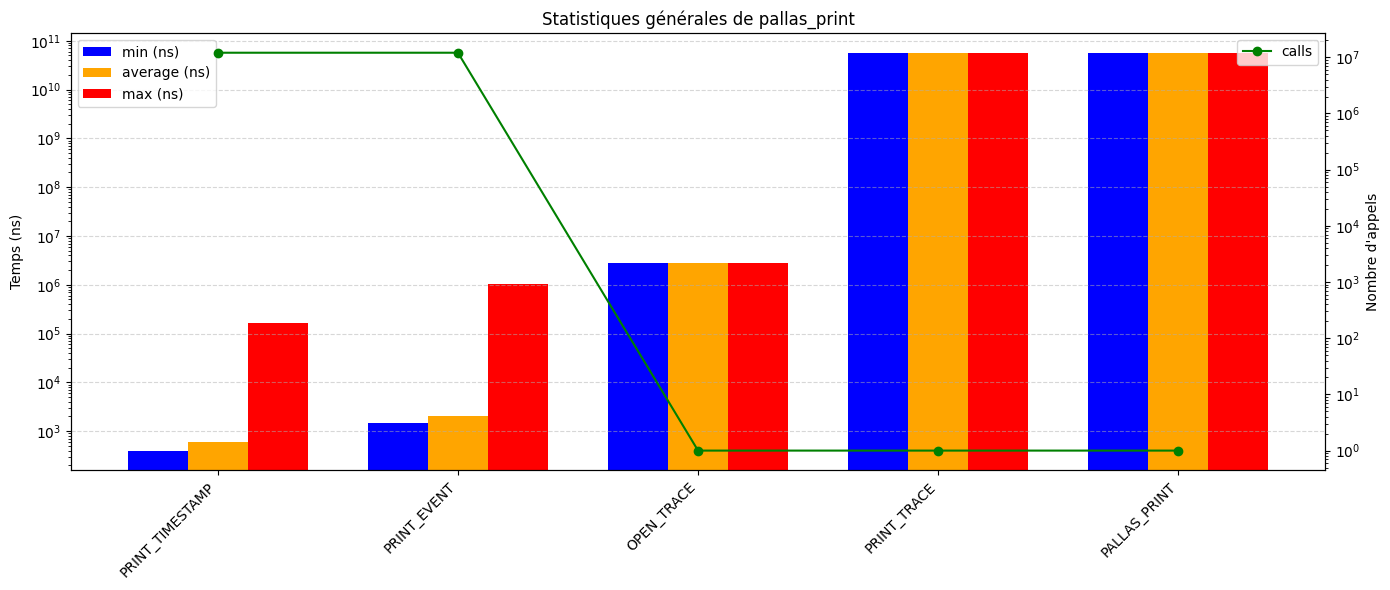
\includegraphics[width=1\textwidth]{img/pallas_print_gen.png}
    \caption{Statistiques générales de pallas\_print}
    \label{fig:pallas_print}
\end{figure}

Parmi les fonctions considérées, on a pallas\_print qui remprésente la durée totale de l'application, open\_trace qui est la durée d'ouverture de la trace,
puis print\_timestamp et print\_event qui sont les durées représentant respectivement l'affichage d'un timestamp et d'un évènement.
Le graphique ci-dessus~\ref{fig:pallas_print} a été réalisé sur une seule observation d'une trace issue du Benchmark NAS LU lancé sur 64 coeurs.

On remarque que la durée d'exécution totale de l'application pallas\_print est issue principalement de la fonction print\_event.

\subsubsection{Solution}\label{ssec:pallas_print_sol}

Ainsi, il faut analyser plus précisément la fonction print\_event.
Pour ce faire, j'ai découpé cette fonction en plusieurs parties. 

On remarque que, à chaque appel à cette fonction, il y a un appel à la fonction \verb!std::endl! de la bibliothèque standard C++. Or celle-ci réalise un flush systématique du buffer sur le disque.
Le fait de faire un flush systématique peut ajouter du temps inutile à l'exécution du programme.
Il est alors possible de remplacer ce \verb!std::endl! par l'écriture simple de \verb!'\n'!.


\begin{figure}[!h]
    \centering
    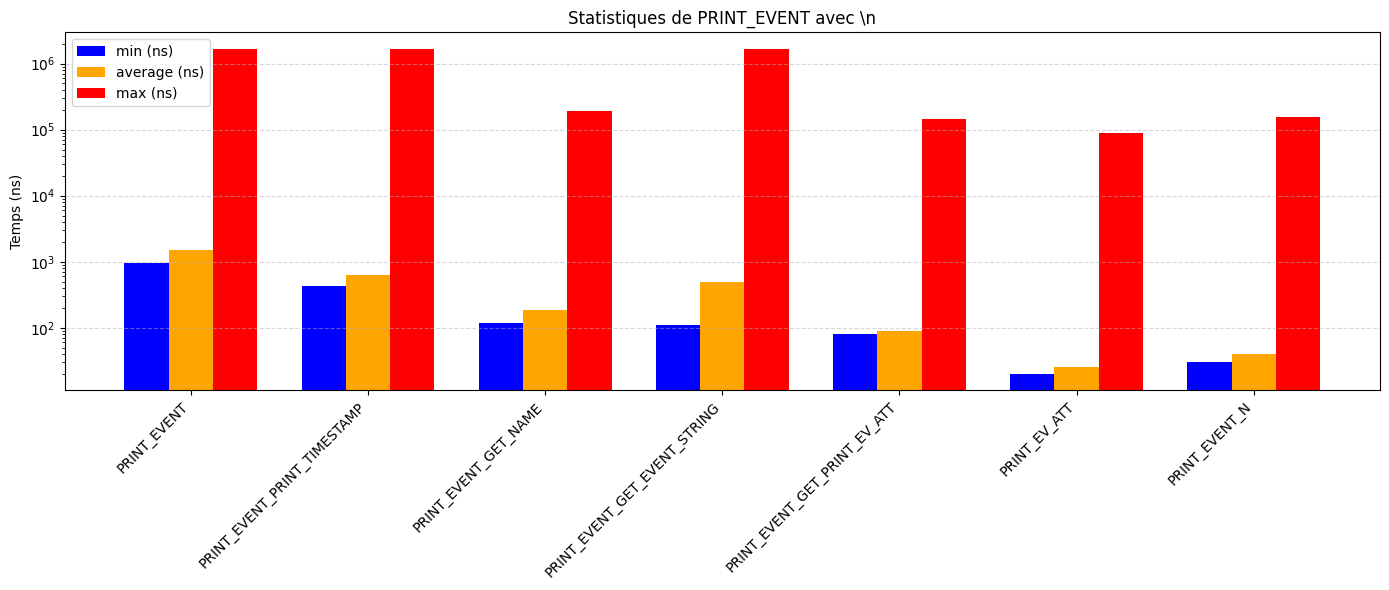
\includegraphics[width=1\textwidth]{img/print_event_n.png}
    \caption{Statistiques détaillées de print\_trace avec un '\textbackslash n'}
    \label{fig:print_event_n}
\end{figure}

\begin{figure}[!h]
    \centering
    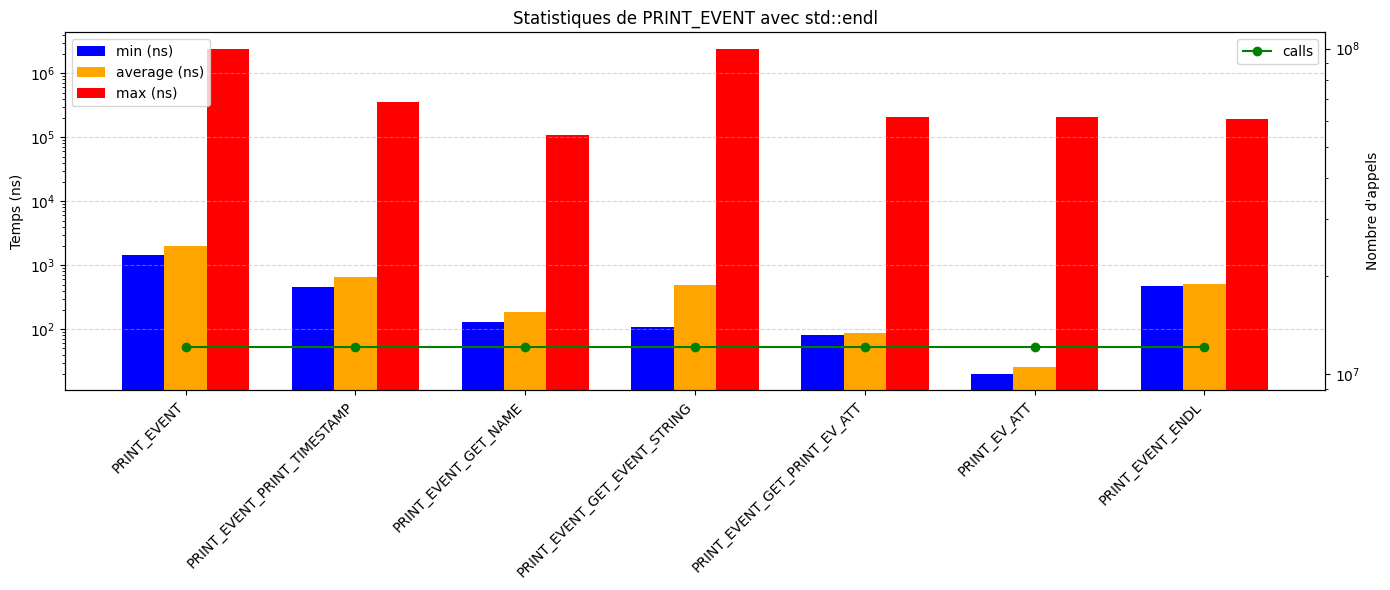
\includegraphics[width=1\textwidth]{img/print_event_endl.png}
    \caption{Statistiques détaillées de print\_trace avec un std::endl}
    \label{fig:print_event_endl}
\end{figure}

Ainsi, sur la figure~\ref{fig:print_event_n} on observe les statistiques de print\_trace avec l'écriture d'un \verb!'\n'! et sur la figure~\ref{fig:print_event_endl} on a les statistiques de print\_trace avec un \verb!std::endl!.
Cette trace ayant 12067968 évènements, on passe d'un temps total par appel à print\_trace à 2000 ns/évènement avec un \verb!std::endl! à 1500 ns/évènement avec l'écriture de \verb!'\n'!, ce qui représente un gain
total de 500 ns/évènement, et dans le cas de cette trace 6 secondes sur le temps d'exécution total.\\
Enfin, c'est une application difficile à analyser et à optimiser car il y a un certain nombre de données à charger avec des copies de structures de dictionnaire.


\subsection{Evaluation de l'overhead induit par PALLAS}\label{ssec:overhead}
\subsubsection{Mise en situation}\label{ssec:overhead_context}

Dans le contexte du calcul haute performance, il est primordial d'utiliser des outils dont l'impact est minimal sur les performances des applications.
C'est ce que l'on va essayer d'évaluer pour l'utilisation de \verb!PALLAS! dans cette partie.

Tout d'abord, il a fallu mettre en place des outils afin de réaliser cette évaluation. Ces outils seront réutilisés dans toute la suite de l'analyse et sont tous dans le repo \cite{pallas-analysis}.

Afin d'installer \verb!PALLAS! avec le traceur \verb!EZTrace!, il y a le script \verb!building_eztrace_pallas.sh! situé dans le dossier \verb!build_pallas_eztrace/!.
Puis, pour lancer les différents benchmarks, il y a les scripts \verb!bash! situés dans le dossier \verb!run_benchmarks! permettant de compiler les différents
exécutables dans un premier temps, puis de lancer les programmes dans un second temps (de plusieurs manières différentes, en fonction des données que l'on veut récupérer et de l'aspect que l'on souhaite étudier).

Dans le cadre de l'étude de l'overhead (temps ajouté au programme initial par l'utilisation de \verb!PALLAS!), on a besoin de récupérer principalement la durée totale de l'exécution du programme.
Pour ce faire, j'ai utilisé la commande \verb!time! de Linux.

\subsubsection{Protocole expérimental}\label{ssec:overhead_exp}

Afin d'analyser l'overhead de manière précise, il a fallu exécuter tous les benchmarks présentés dans la partie~\ref{ssec:outils} de ce rapport, avec et sans \verb!EZTrace!.
Ces benchmarks ont été itérés 20 fois pour plus de précision.

De plus, il a fallu récupérer ces données d'exécution dans les fichiers de log de ces derniers et enfin les tracer à l'aide de la bibliothèque \verb!matplotlib! de \verb!Python!.
Afin d'uniformiser les barres relatives à chaque application, les valeurs de ces dernières ont normalisées par les données de l'application Vanilla (sans tracé).

\subsubsection{Résultats}\label{ssec:overhead_res}

\begin{figure}[!h]
    \centering
    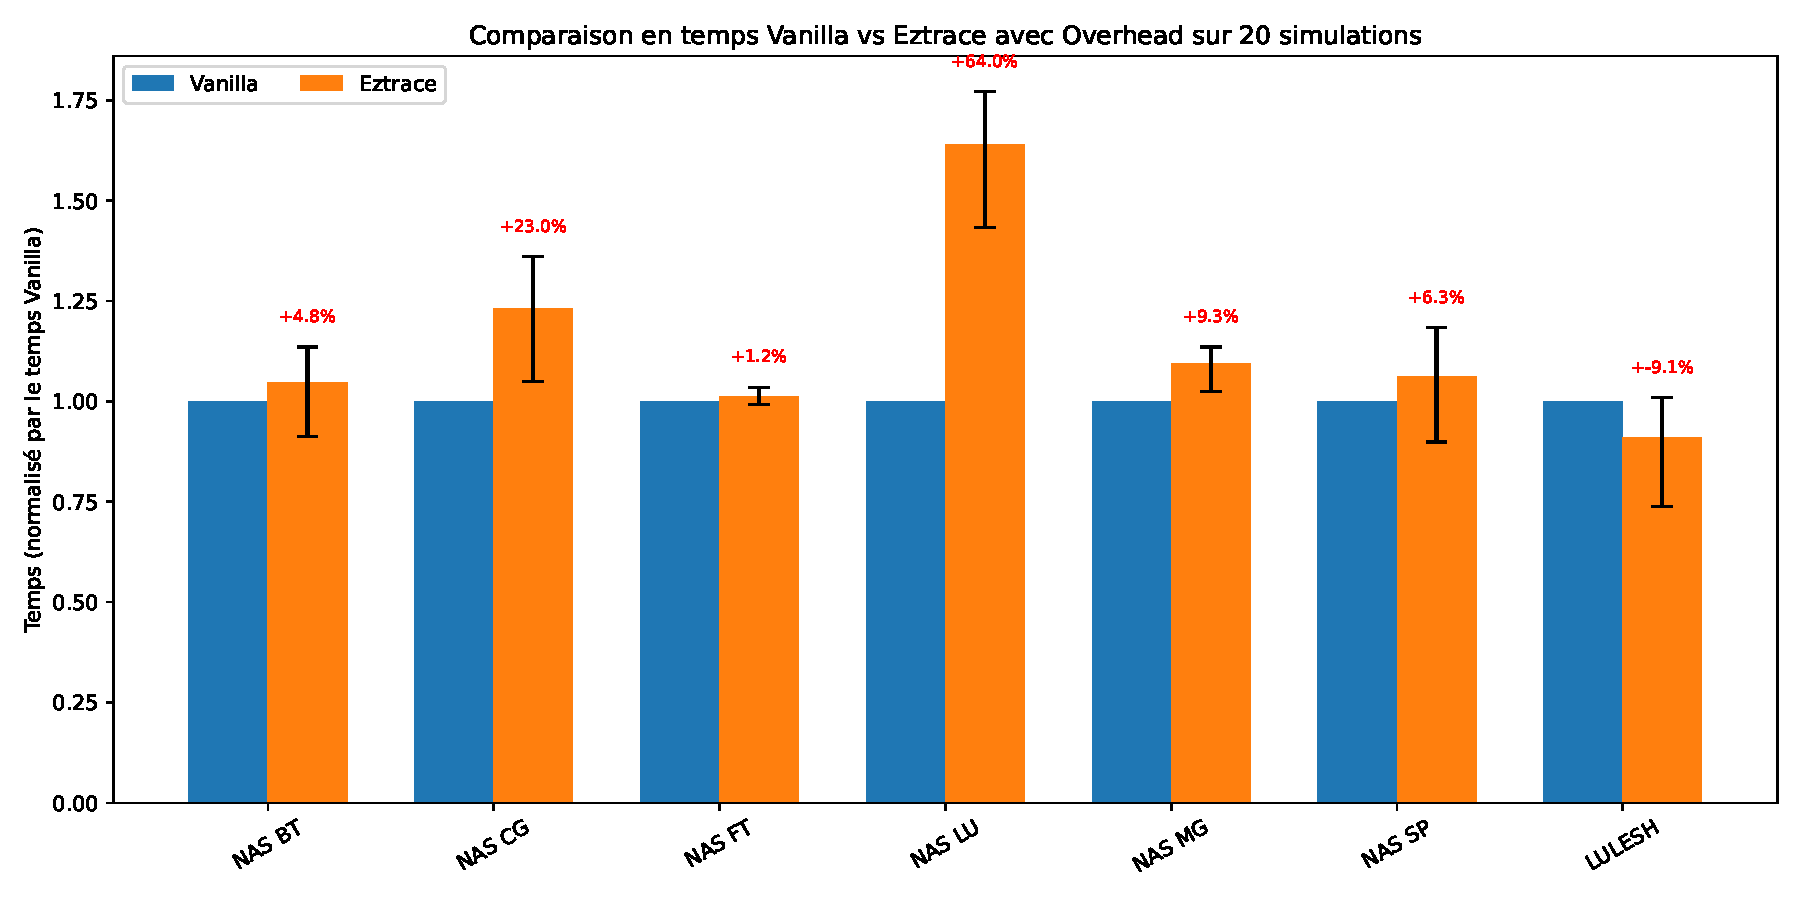
\includegraphics[width=1\textwidth]{img/overhead.pdf}
    \caption{Overhead généré par EZTrace/PALLAS}
    \label{fig:overhead}
\end{figure}

Les résultats de l'overhead induit par le tracé de \verb!EZTrace! sont représentés dans le graphique~\ref{fig:overhead}.
On constate que dans les cas comme \verb!NAS BT!, \verb!NAS FT!, \verb!NAS MG!, \verb!NAS SP! et \verb!LULESH!, on a un impact inférieur à 10\% du temps total d'exécution de l'application.
Dans les cas des benchmarks \verb!NAS BT! et surtout \verb!NAS LU! on a un impact significatif sur le temps d'exécution total de l'application qui atteint un maximum de 64\%.
Ainsi, on peut conclure que dans les cas d'applications très régulières, l'overhead induit par l'utilisation de \verb!PALLAS! avec \verb!EZTrace! reste suffisament négligeable.

\subsection{Analyse de la compression et de l'écriture sur les disque de PALLAS}\label{ssce:wrt_write}

\subsubsection{Situation actuelle}\label{ssec:wrt_situ}

\verb!PALLAS! enregistre les différentes données d'exécution sous forme de listes doublement chainées, décomposées en sous-listes dont la taille est fixée.
Tout le vecteur est stocké en mémoire et écrit d'un seul coup sur les disques en fin d'exécution.
L'algorithme de compression retenu par défaut est \verb!ZSTD! qui est un algorithme sans pertes.

\subsubsection{Methodes d'analyse}\label{ssec:wrt_analysis}

Un facteur intéressant à faire varier est la taille des sous-vecteurs permettant de stocker les données. Par défaut, celle-ci est fixée à \verb!1000!.
Afin, de les faire varier, j'ai appliqué des patchs git (qui permettent d'enregistrer différents commits) à la taille de ces sous-vecteurs.
Les tailles testées sont \verb!100!, \verb!1000!, \verb!10000!, \verb!100000!, \verb!500000!, \verb!1000000!.
Les données recueillies sont les statistiques sur le temps d'écriture et de compression (par fonctions puis par parties de fonctions) lors de l'exécution
d'un programme avec différentes tailles de vecteurs.
Puis des graphiques sont réalisés grace à des scprits \verb!python! qui permettent d'aggréger les données. 

\subsubsection{Résultats obtenus}\label{ssec:wrt_res}

\begin{figure}[!h]
    \centering
    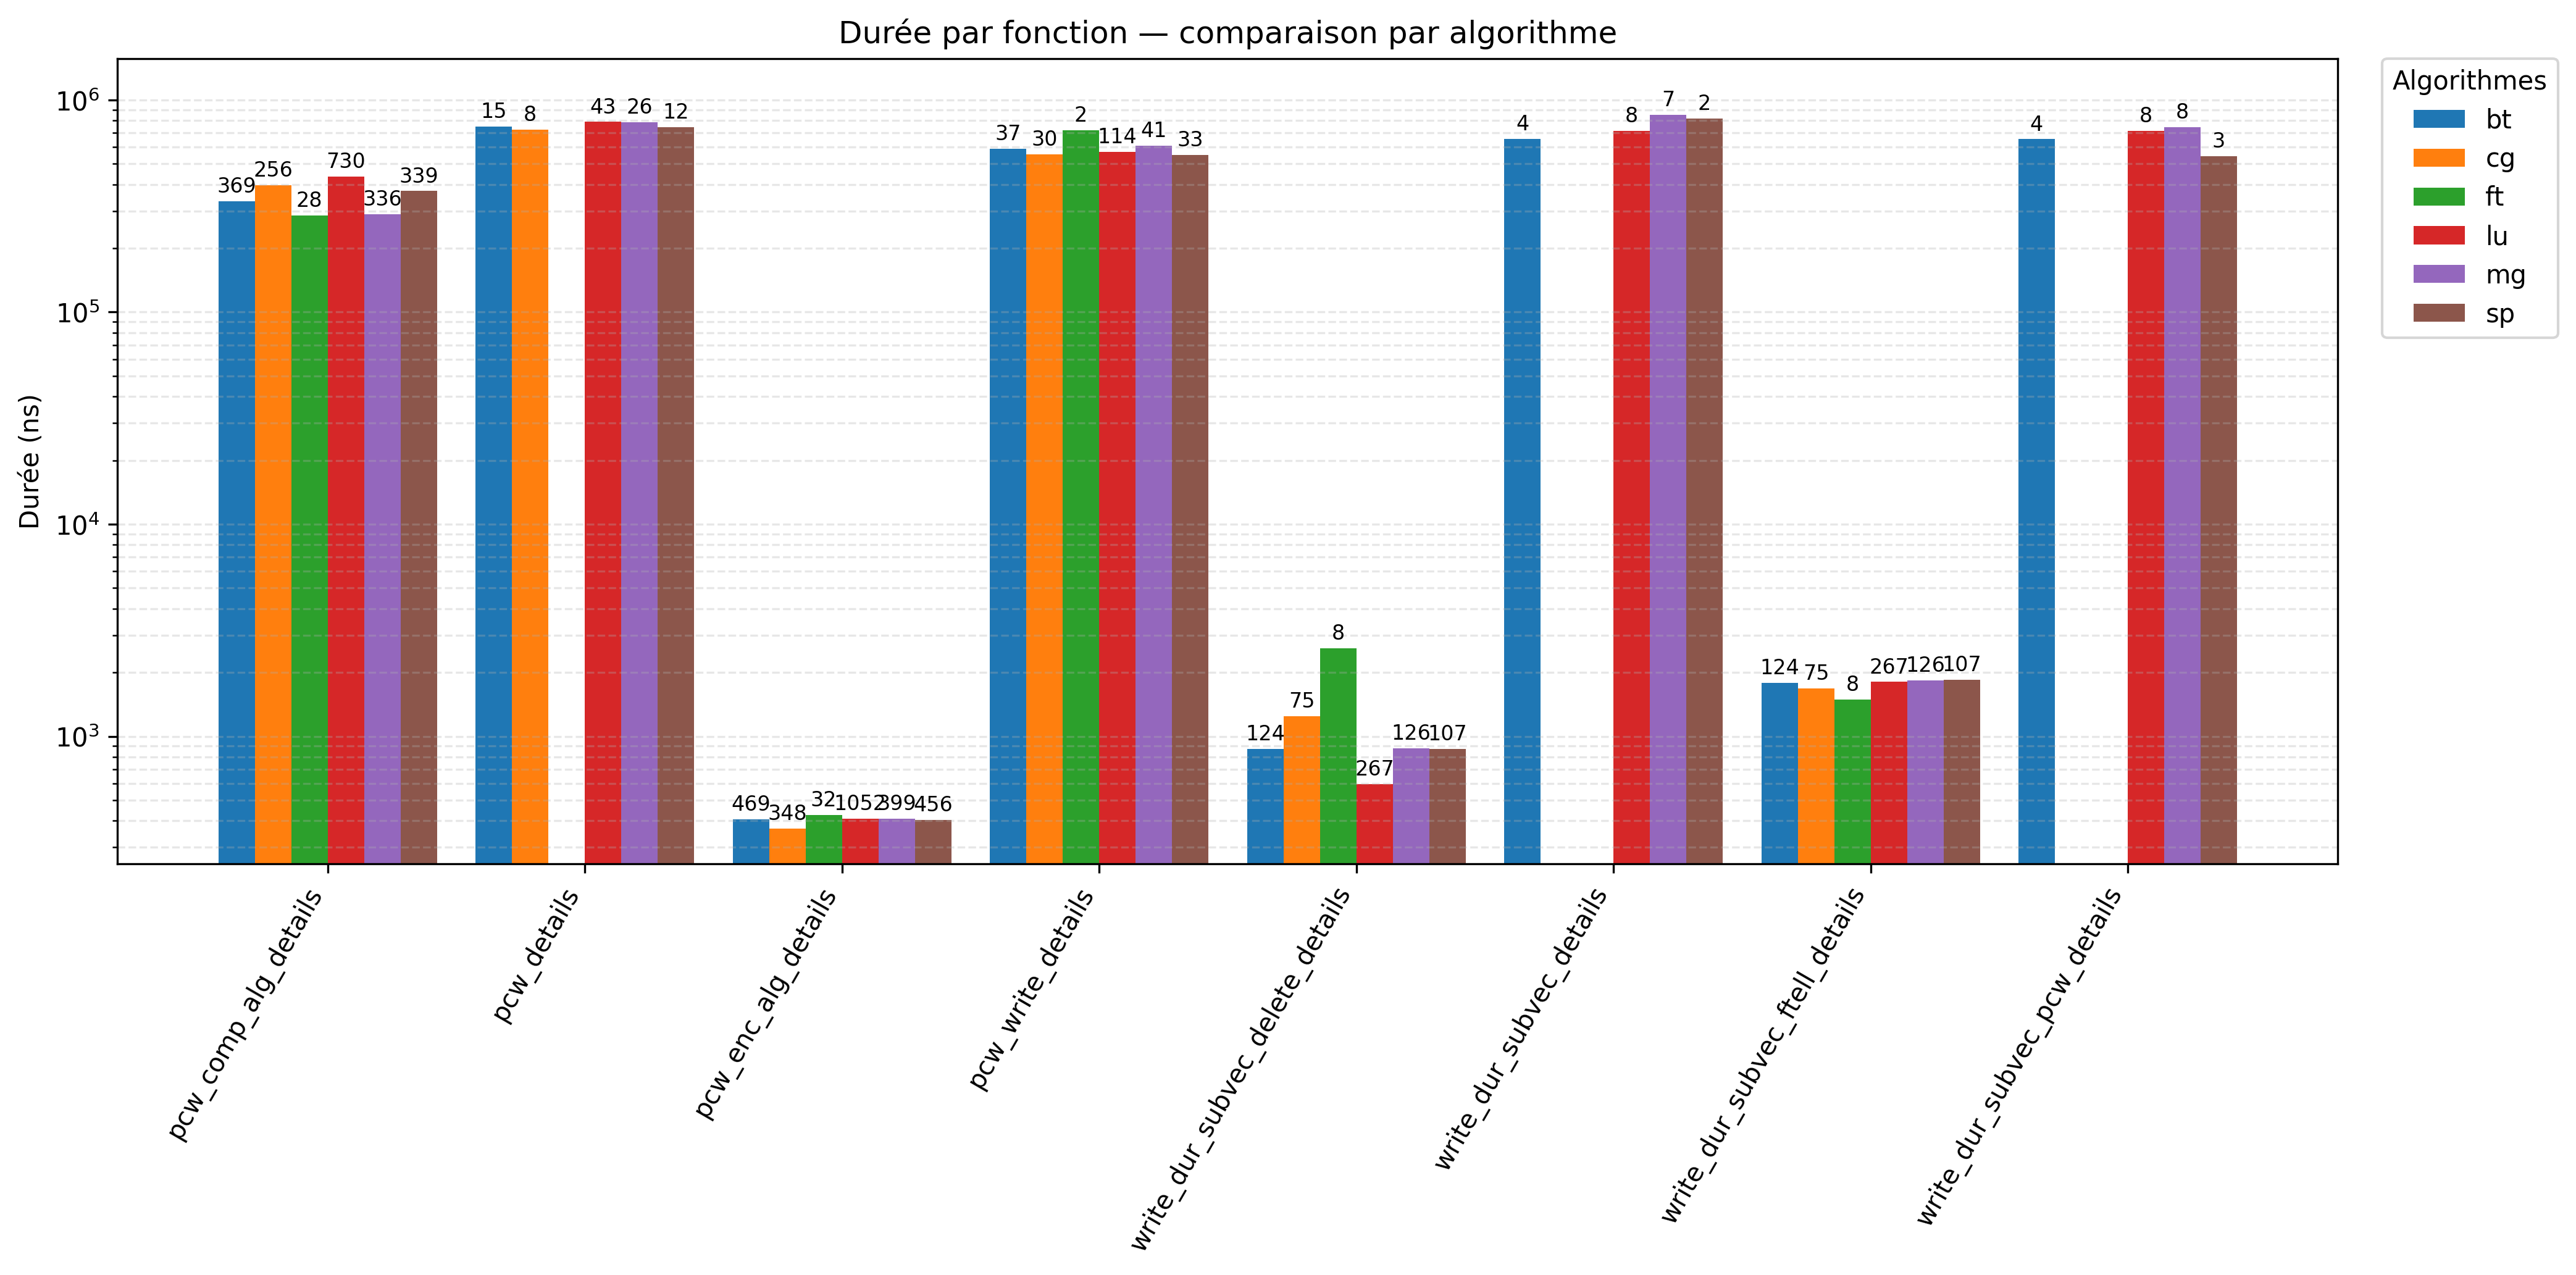
\includegraphics[width=1\textwidth]{img/pcw_global.png}
    \caption{Durées générales de l'écriture et de la compression}
    \label{fig:pcw_global}
\end{figure}
\begin{figure}[!h]
    \centering
    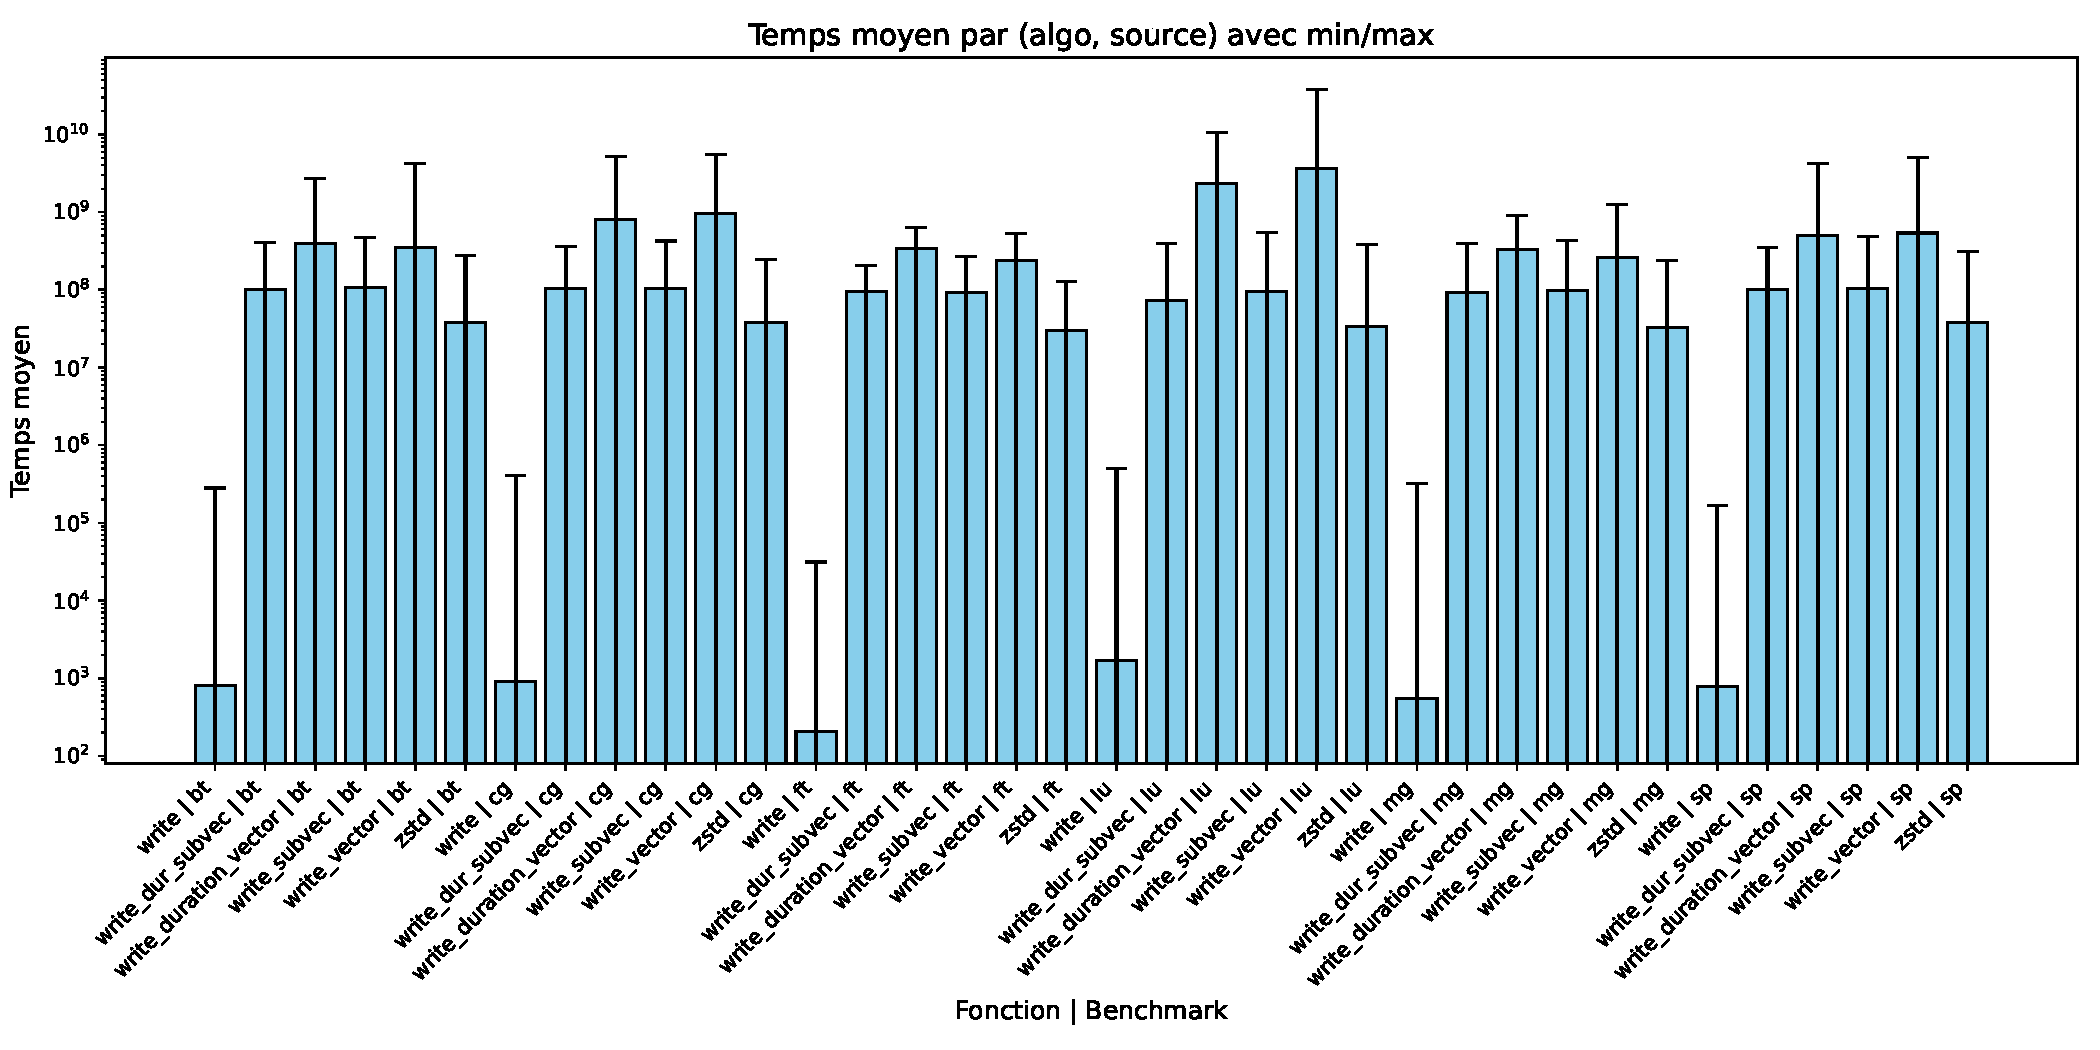
\includegraphics[width=1\textwidth]{img/nas_comp_write.pdf}
    \caption{Fonctions d'écriture et de compression}
    \label{fig:cw_global}
\end{figure}
Tout d'abord, l'écriture sur le disque ainsi que la compression des données sont réalisés par la fonction \verb!pallas_compress_write! (abrégé par pcw dans le graphique~\ref{fig:pcw_global}),
donc avant de lancer les programmes sur différentes tailles de sous-vecteurs, il faut observer cette fonction là.
Le nombre d'appels à chaque fonction dans chacun des benchmarks est écrit au dessus de chaque barre.\\
On remarque que le temps total de la fonction de compression et d'écriture est dû principalement à la fonction d'écriture ainsi que celle de compression.

De plus, d'après le graphique~\ref{fig:cw_global}, on observe que ce sont les fonctions \verb!write_vector! et \verb!write_duration_vector! (qui écrivent respectivement les vecteurs de timestamps et de durées)
qui prennent le plus de temps.\\
\begin{figure}[!h]
    \centering
    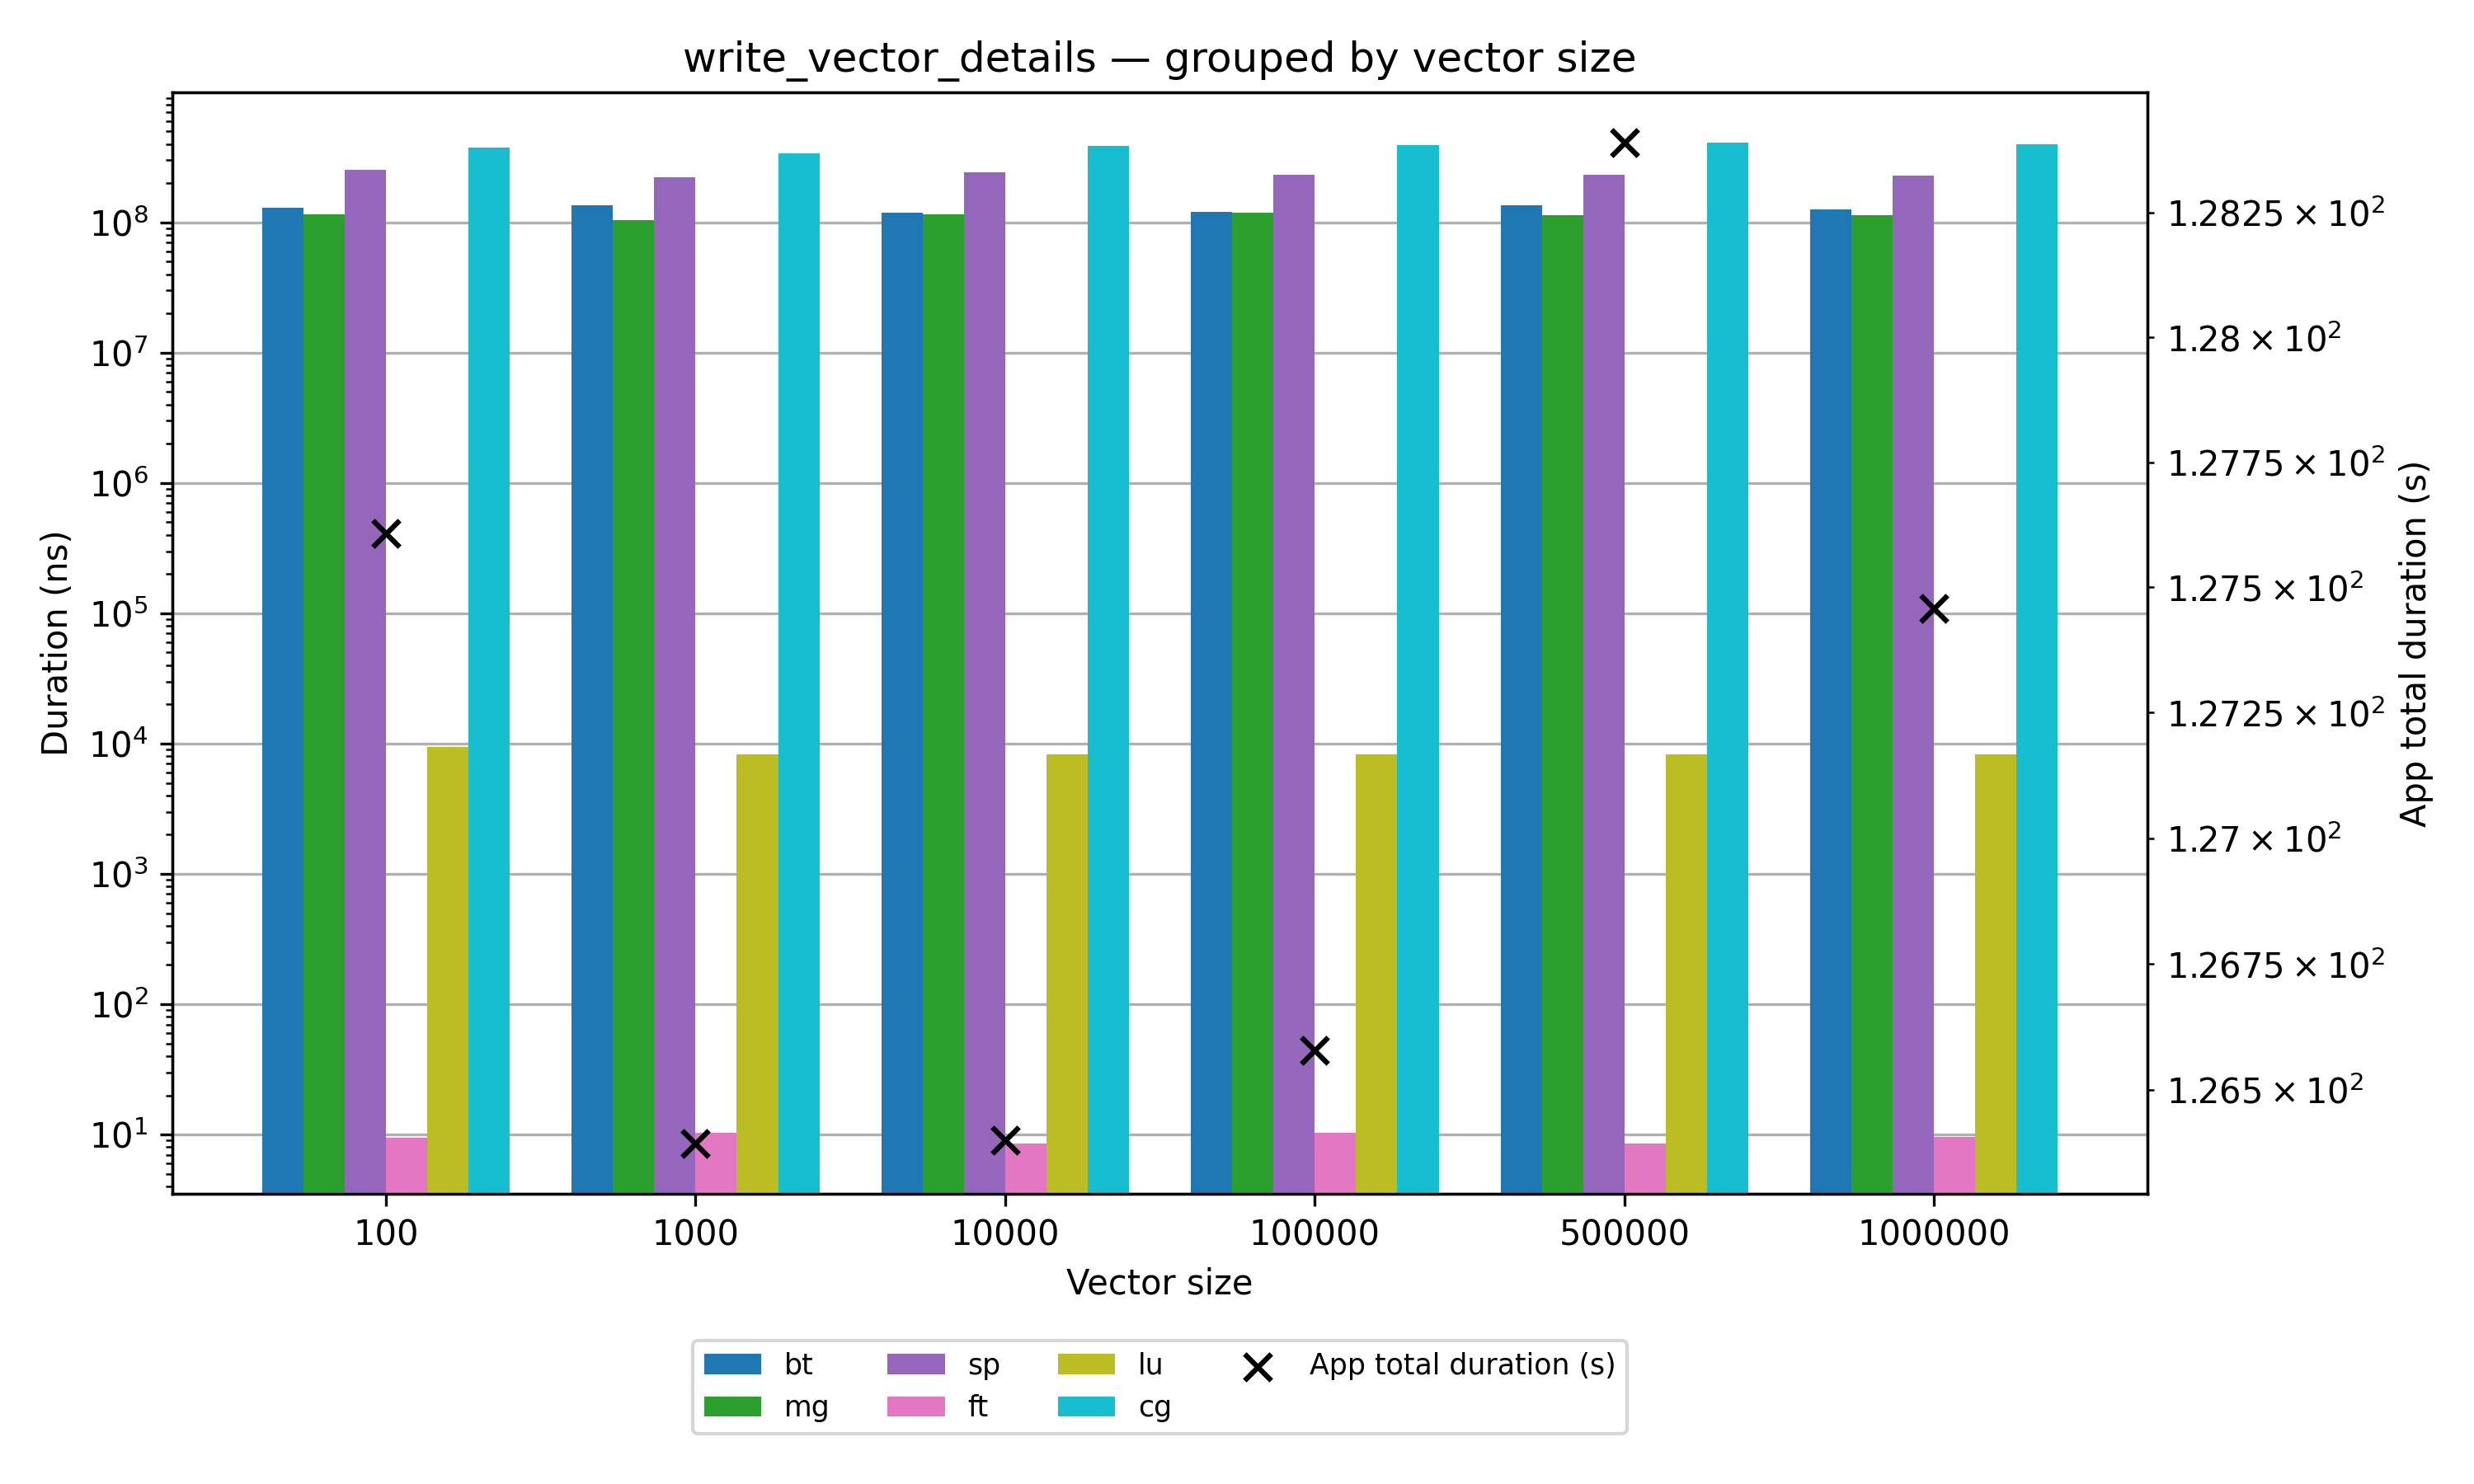
\includegraphics[width=1\textwidth]{img/write_vector_details.png}
    \caption{Statistiques des durées de l'écriture d'un vecteur}
    \label{fig:a}
\end{figure}
\begin{figure}[!h]
    \centering
    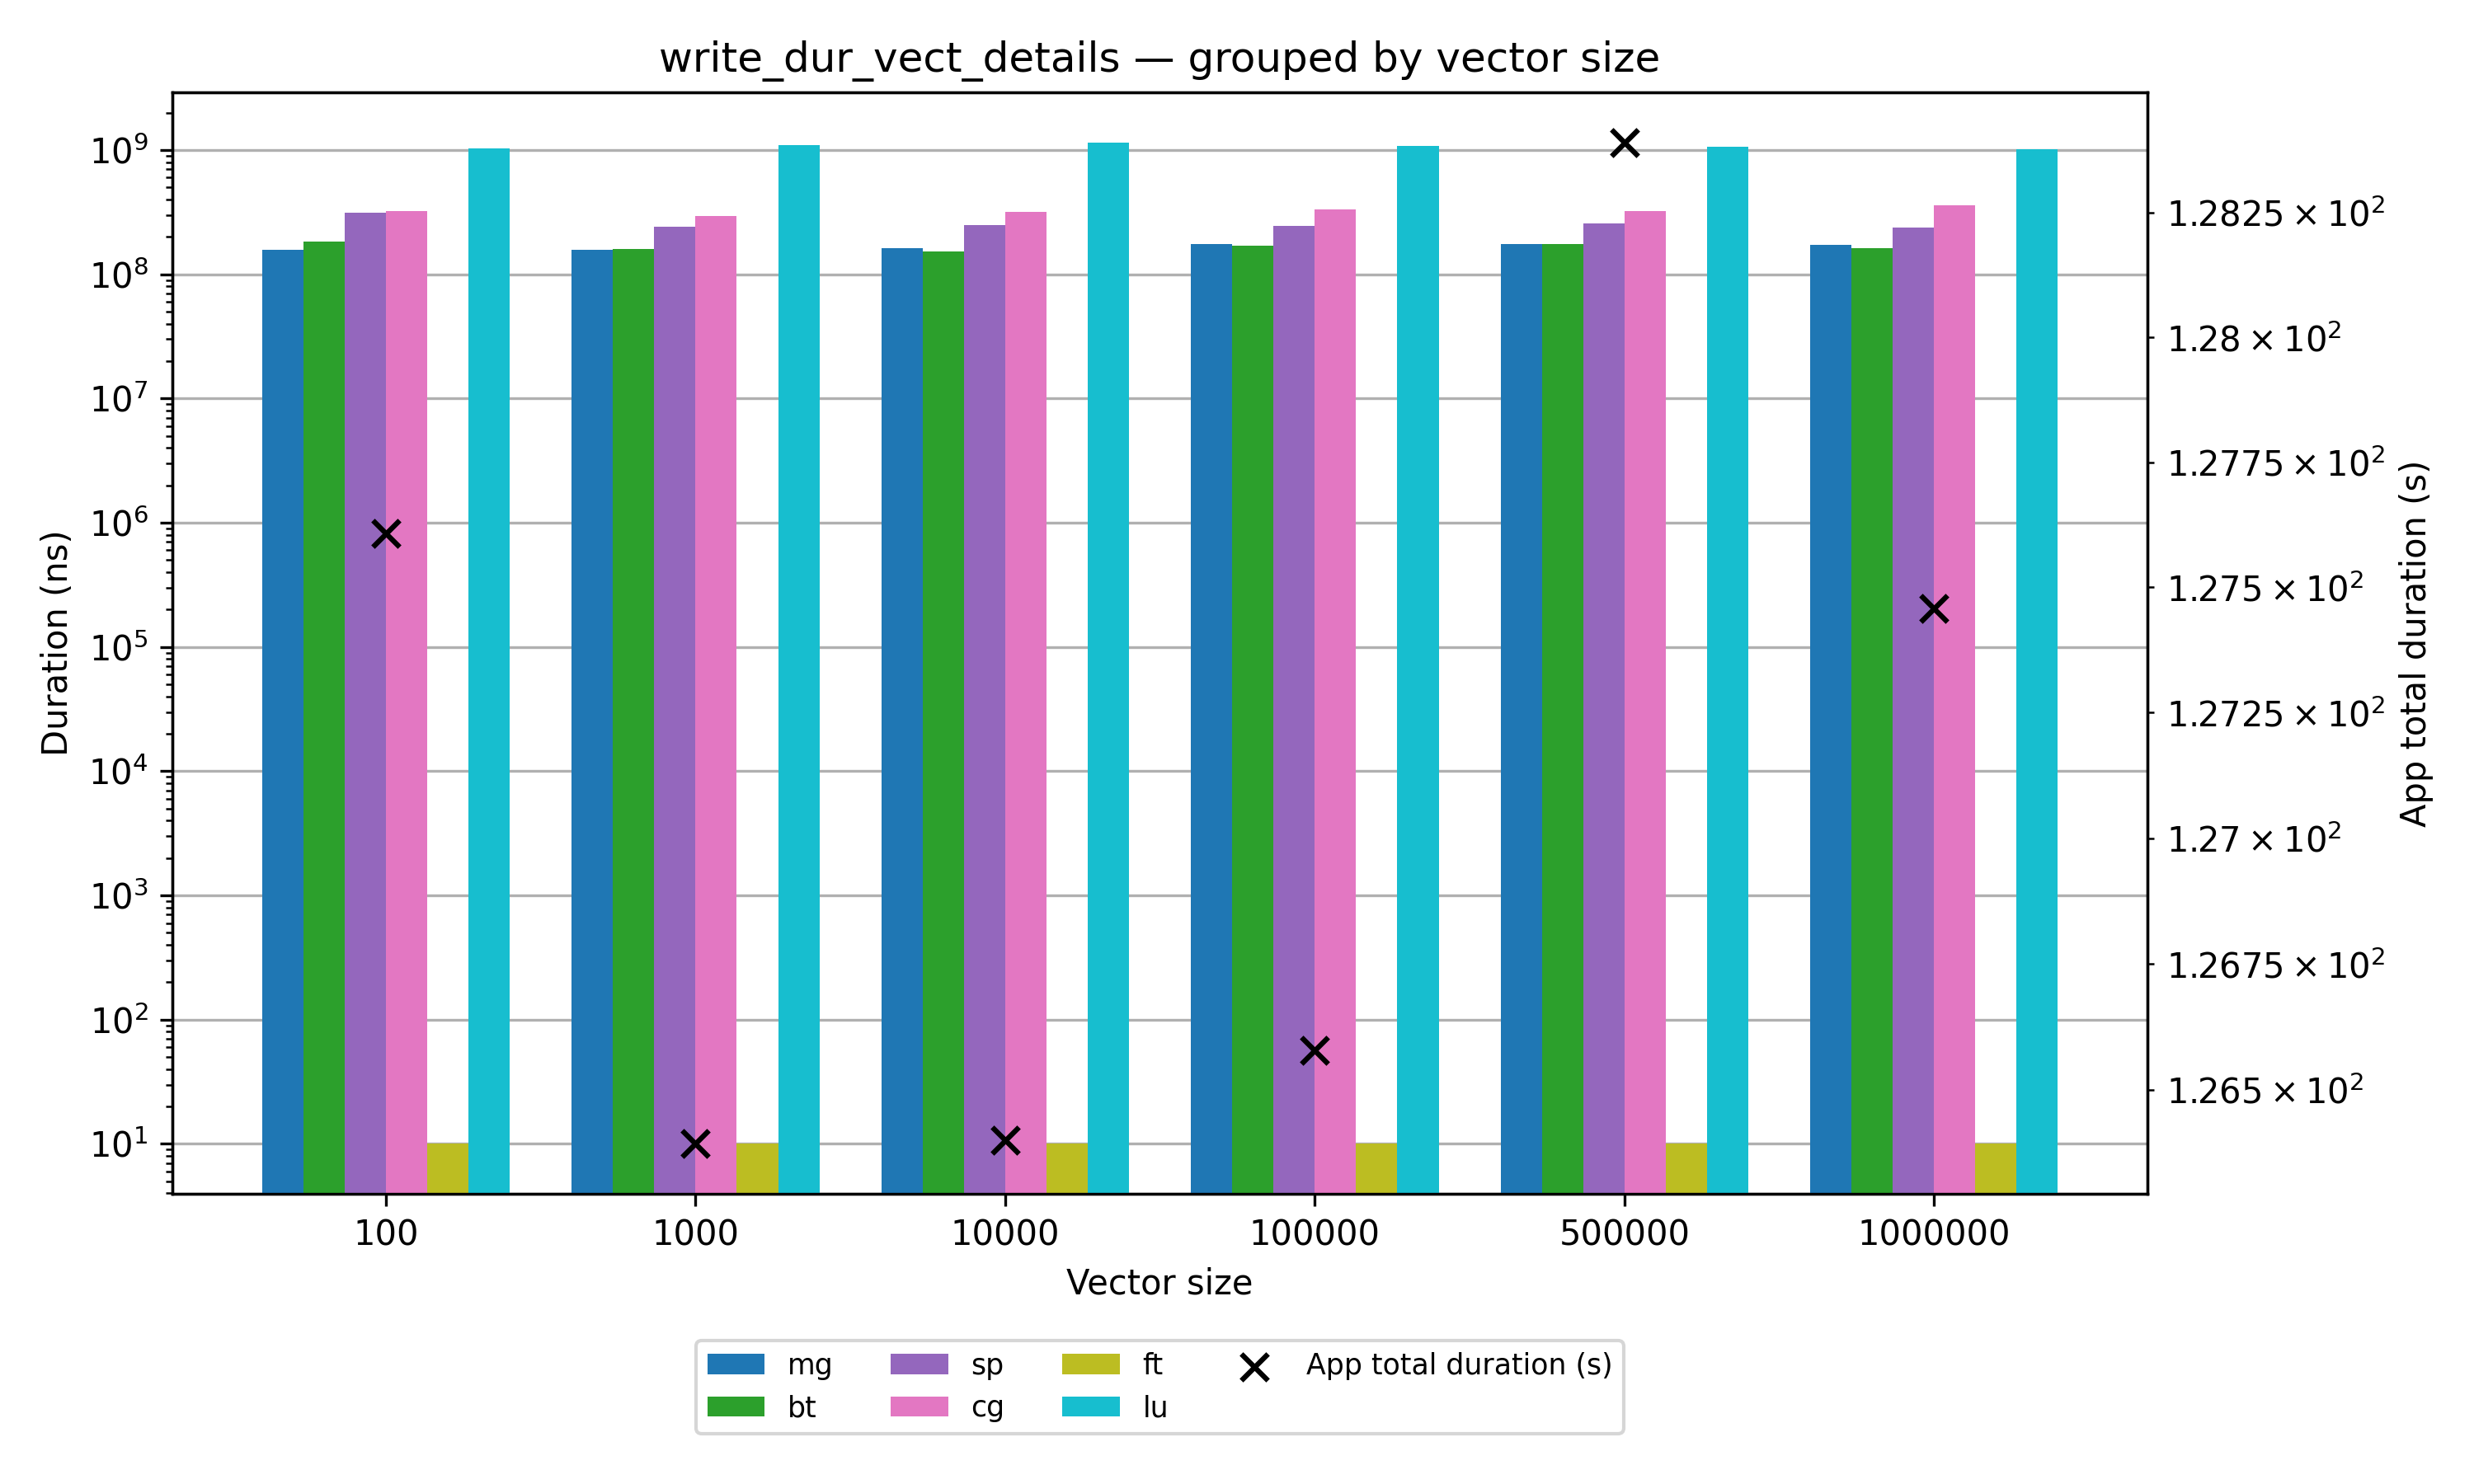
\includegraphics[width=1\textwidth]{img/write_dur_vect_details.png}
    \caption{Statistiques des durées d'écriture d'un vecteur de durées}
    \label{fig:b}
\end{figure}
\begin{figure}[!h]
    \centering
    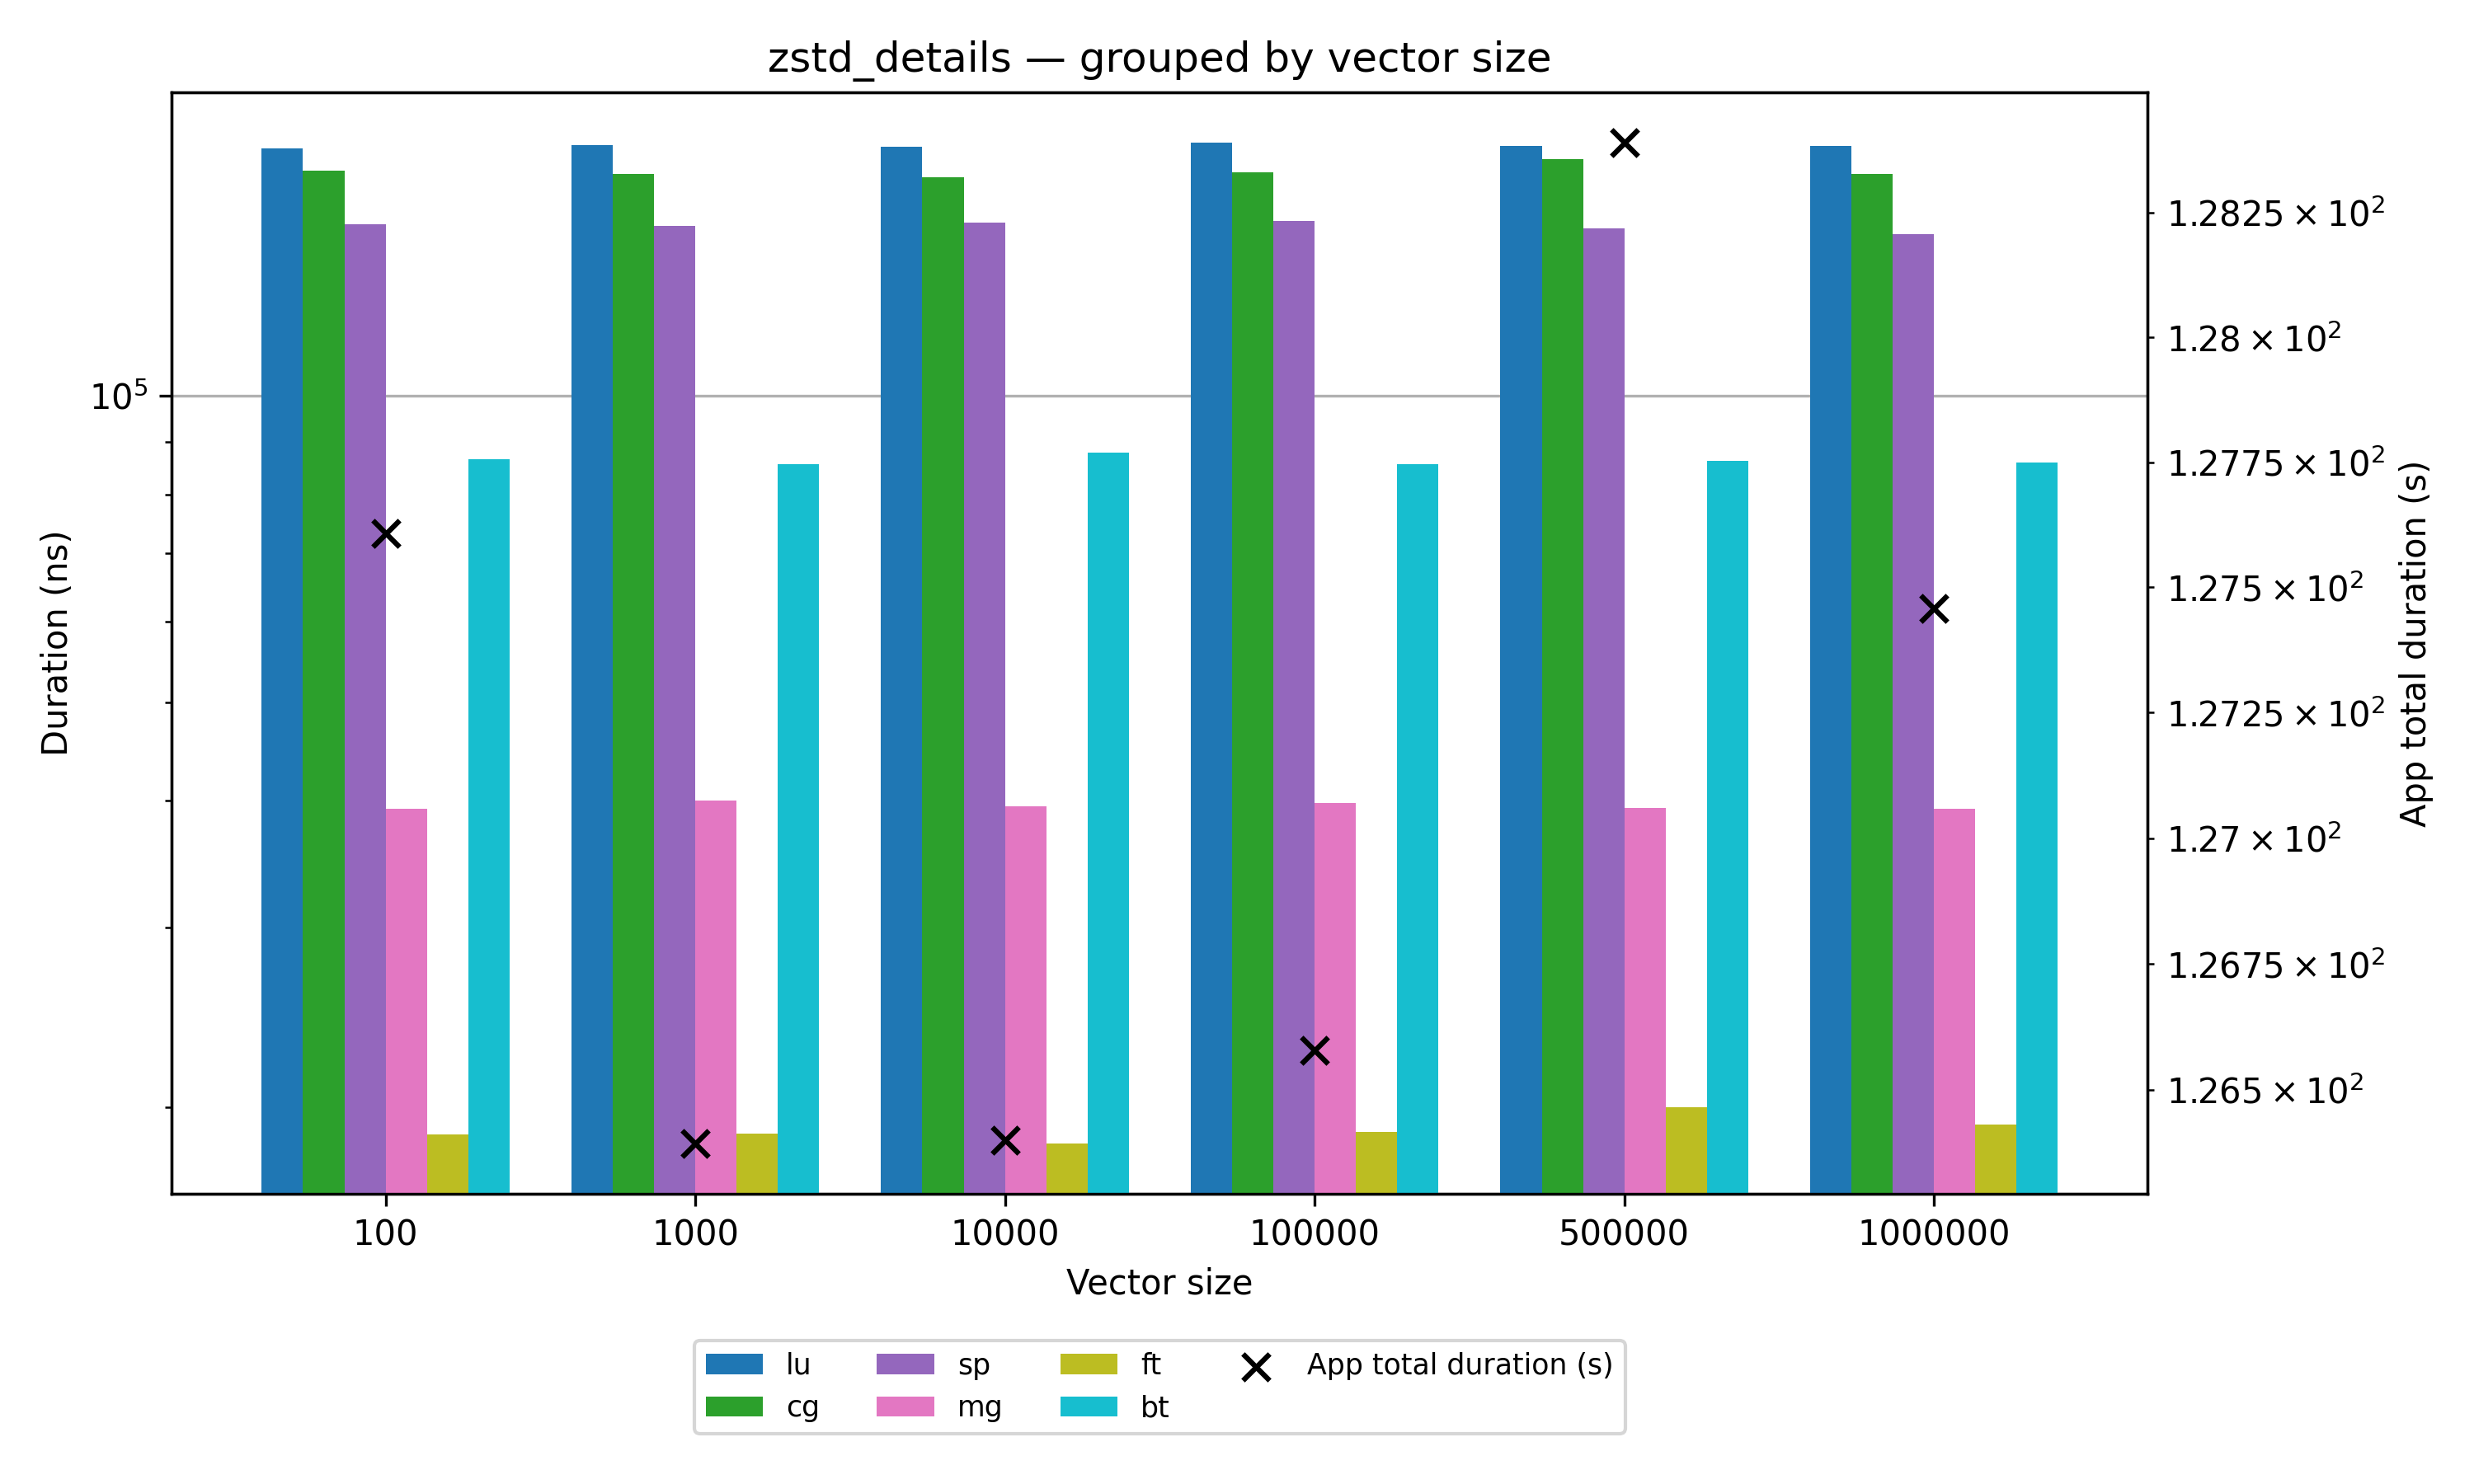
\includegraphics[width=1\textwidth]{img/zstd_details.png}
    \caption{Statistiques de durée de la compression d'un vecteur}
    \label{fig:c}
\end{figure}
\begin{figure}[!h]
    \centering
    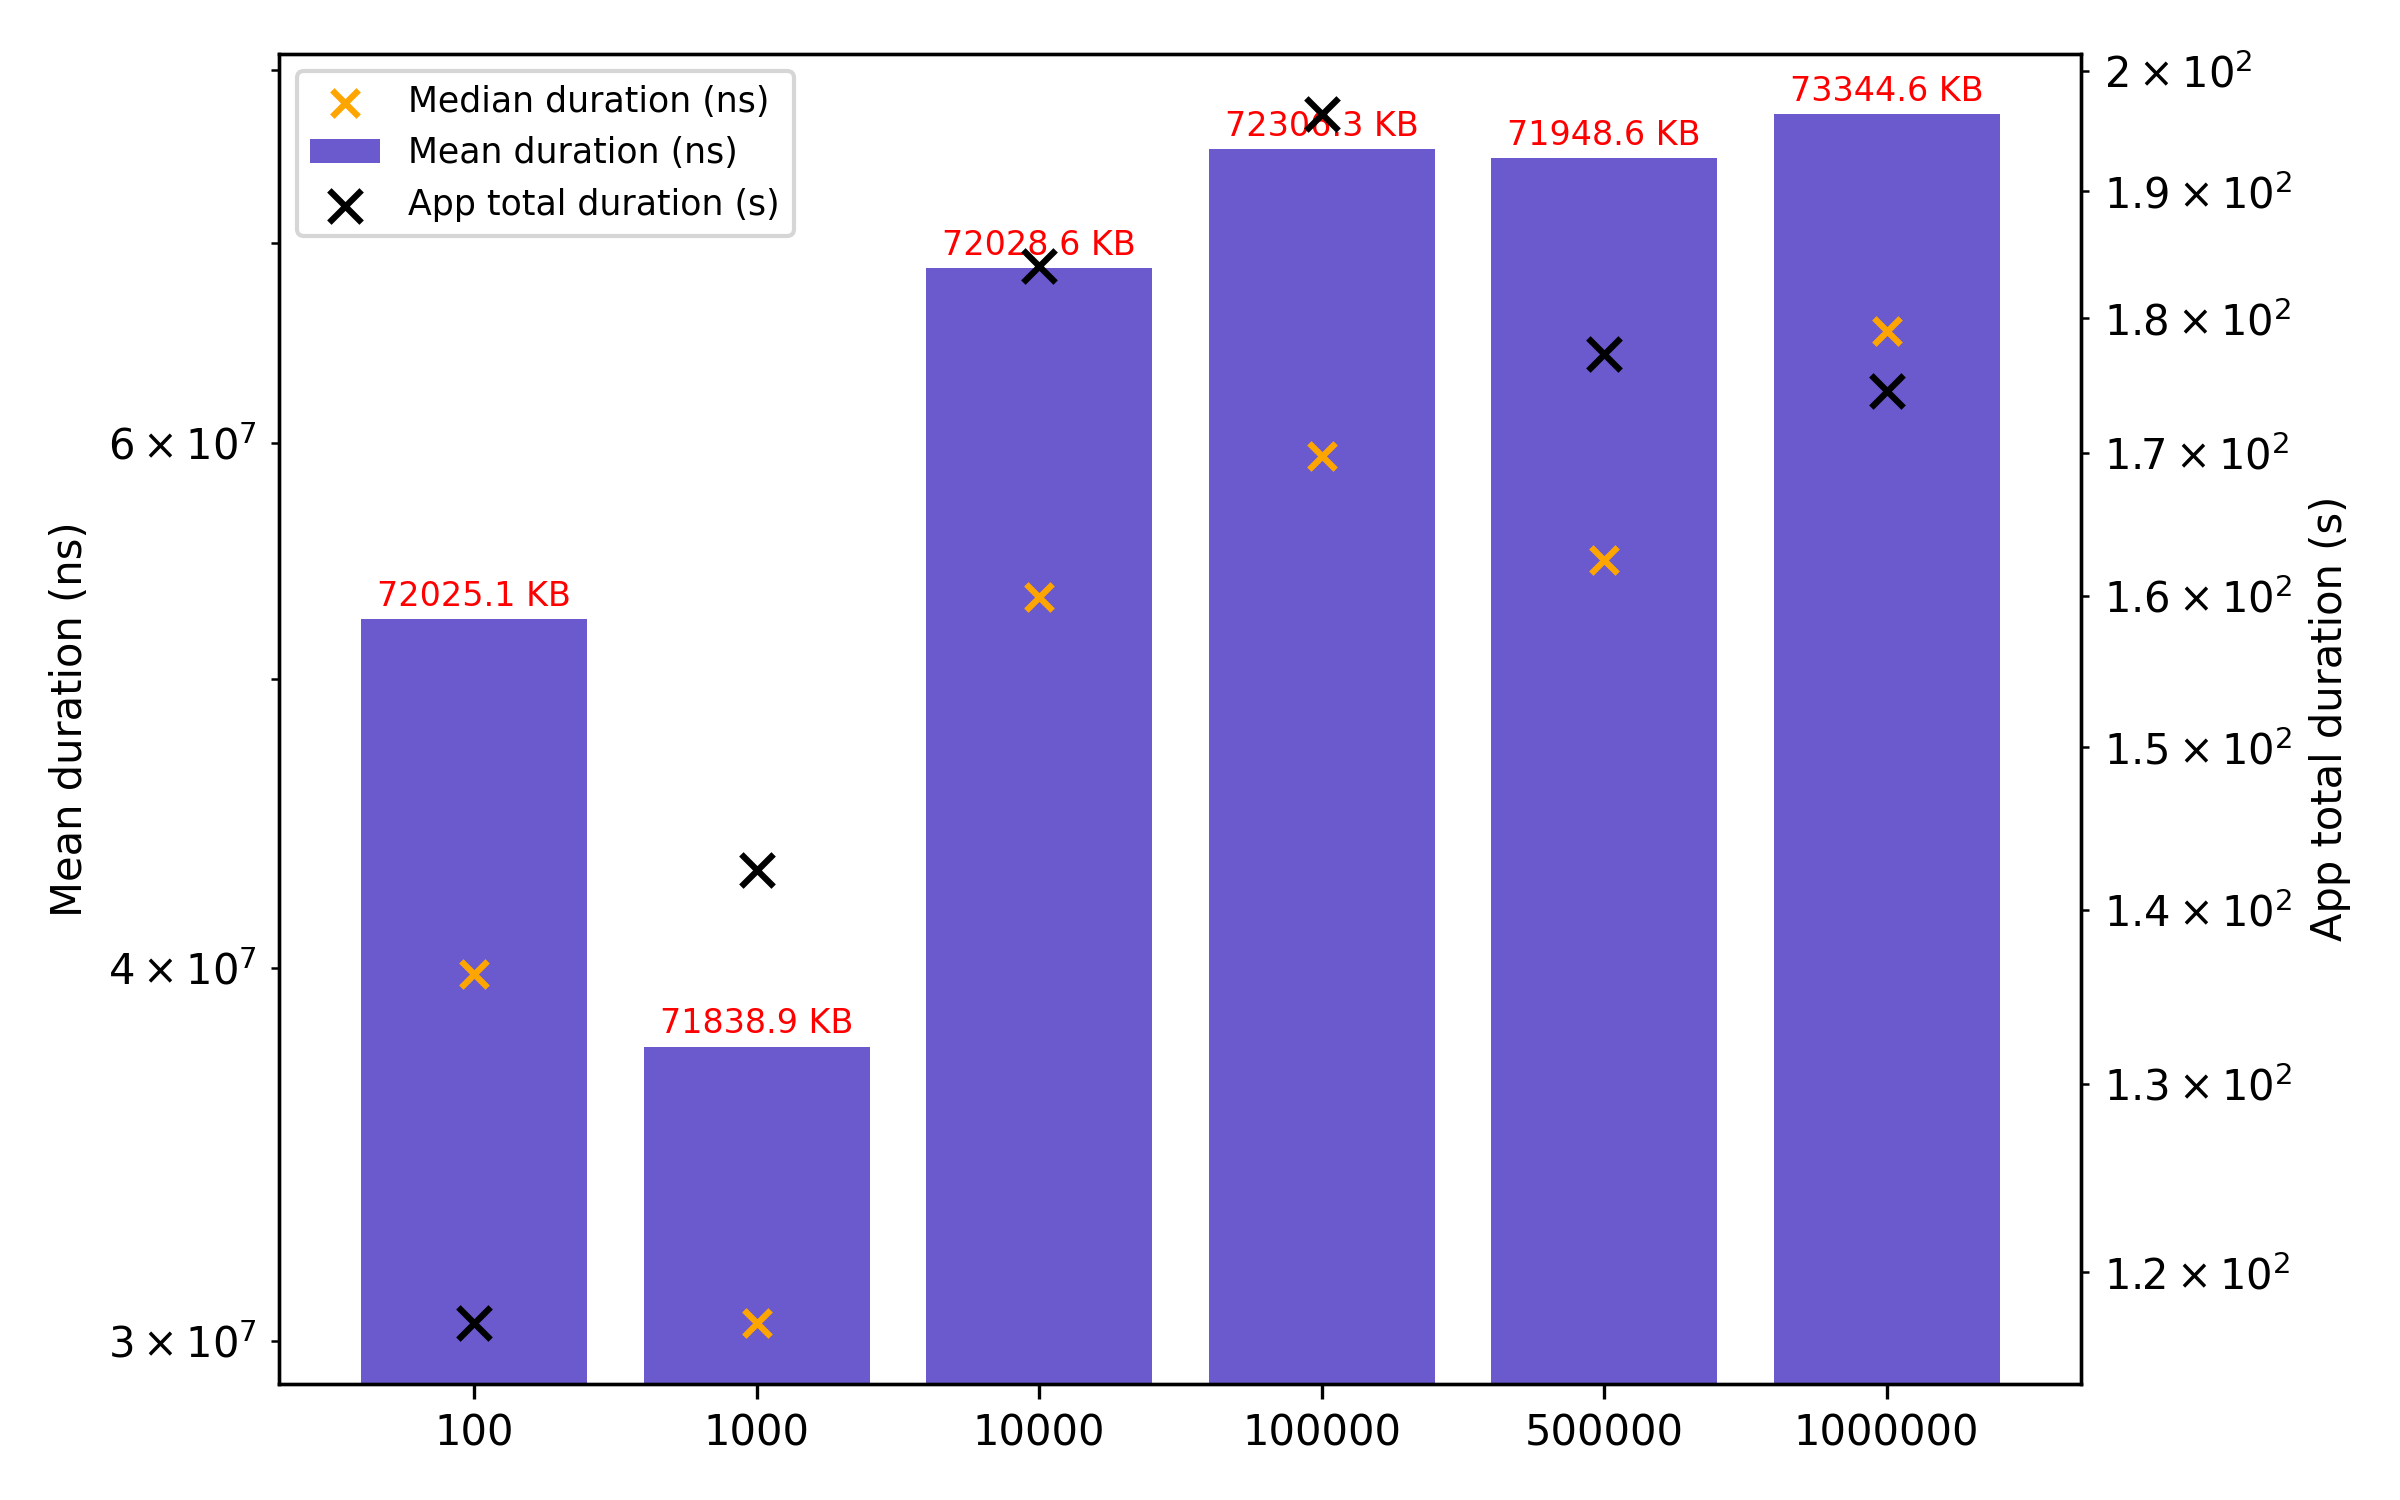
\includegraphics[width=1\textwidth]{img/write_dur_subvec_bof.png}
    \caption{Moyennes des durées d'écriture d'un vecteur de durées}
    \label{fig:d}
\end{figure}
Dans le graphique~\ref{fig:d}, une moyenne a été réalisée sur toutes les applications observées par taille de sous-vecteur et par fonction observée (ici l'écriture d'un vecteur de durées a été observée).
On remarque alors que c'est pour une taille de sous-vecteur de \verb!1000!, c'est-à-dire la longueur par défaut que l'on a les meilleurs résultats. 
En rouge, on observe également le pic mémoire lors des différentes exécutions, qui est assez stable mais minime pour la taille de \verb!1000!.
Mais ce graphique est à relativiser car une moyenne non pondérée a été faire alors que les différentes traces ont des tailles extrêmement variées.

Enfin, pour la comparaison des comportements des fonctions les plus coûteuses en fonction de la taille des sous-vecteurs (écriture et compression de ces derniers),
on retrouve les résultats dans les graphiques~\ref{fig:a},~\ref{fig:b} et~\ref{fig:c}.

On observe alors que la variation des tailles de sous-vecteurs n'a pas un impact marquant sur ces fonctions. Par contre, grâce aux croix noires sur ces graphiques qui représentent le temps d'exécution total du programme,
on constate que la taille des sous-vecteurs a tout de même un impact sur le temps d'exécution total (de l'ordre de 2 secondes pour les application observées).

Au final, même si la taille des sous-vecteurs n'a pas un grand impact sur l'application, la taille fixée à \verb!1000! semble être optimale.


\clearpage


\subsection{Etude de différents algorithmes de compression}\label{ssec:comp}
\subsubsection{Situation actuelle}\label{ssec:comp_situ}

L'algorithme de compression choisi par défaut est \verb!ZSTD! qui est sans perte, c'est-à-dire qu'il garantit une restitution parfaite des données, sans erreurs.
Mais \verb!PALLAS! propose d'autres algorithmes tels que \verb!ZFP! qui sont "lossy", c'est-à-dire avec une certaine proportion de perte autorisée.
L'objectif est d'évaluer la perte d'information de ces algoritmes ainsi que leur efficacité.

\subsubsection{Outils mis en place}\label{ssec:comp_tools}

La problématique dans le fait d'évaluer la perte d'information liée à différents algorithmes a été la mise en place d'un outil permettant cette étude.
La solution retenue a été de générer une trace avec \verb!EZTrace! et \verb!PALLAS! et d'utiliser l'application \verb!pallas_editor! qui permet, à partir d'une trace
existante, d'en créer une nouvelle avec un autre algorithme de compression. Ainsi, on peut comparer des traces identiques avec des algorithmes de compression différents.

En suite, les applications \verb!pallas_getTimestamps! et \verb!pallas_durations! ont été mises en place. La première permet de récupérer, à partir d'une trace, un fichier \verb!.csv! avec 
tous les timestamps de cette dernière, récupérés thread par thread. La seconde réalise le test statistique $R^2$ sur deux échantillons de timestamps (la version sans compression sert d'échantillon
de référence).

Ces des applications n'ont pas pu être regrouppées en une seule car l'architecture actuelle de \verb!PALLAS! ne permet pas de parcourir deux fois la même trace de cette manière 
(une partie de ce problème a été résolue car initialement il était impossible d'ouvrir deux traces différentes au même endroit).

\subsubsection{Résultats obtenus}\label{ssec:comp_res}

Les données récoltées ont été classées dans les tables~\ref{lu},~\ref{bt} et \ref{cg} et permettent comparer les différents algorithmes de compression pour les quelques benchmarks considérés
(\verb!NAS LU!, \verb!NAS BT! et \verb!NAS CG!).
Les différents algorithmes de compression étudiés sont l'absence de compression (\verb!None!), \verb!ZSDT!, et l'algorithme \verb!ZFP! avec plusieurs seuils de tolérence différents 
(\verb!0.1!, \verb!0.2!, \verb!0.3!).

% ---------- LU ----------
\begin{table}[h]
\centering
\caption{Résultats LU}\label{lu}
\begin{adjustbox}{max width=\linewidth}
\begin{tabular}{lrrrrr}
\hline
\textbf{Valeur} & \textbf{None} & \textbf{ZSTD} & \textbf{ZFP\_0.1} & \textbf{ZFP\_0.2} & \textbf{ZFP\_0.5} \\
\hline
$R^2$                     & 1            & 1            & 1             & 1             & 1 \\
trace\_size\_MB           & 168          & 67           & 93            & 93            & 93 \\
compression\_duration\_ns & 0            & 1.84647e+09  & 1.48667e+09   & 1.50095e+09   & 1.52376e+09 \\
write\_duration\_ns       & 2.61871e+08  & 1.56096e+08  & 1.90319e+08   & 1.98531e+08   & 1.96283e+08 \\
\hline
\end{tabular}
\end{adjustbox}
\end{table}

% ---------- BT ----------
\begin{table}[h]
\centering
\caption{Résultats BT}\label{bt}
\begin{adjustbox}{max width=\linewidth}
\begin{tabular}{lrrrrr}
\hline
\textbf{Valeur} & \textbf{None} & \textbf{ZSTD} & \textbf{ZFP\_0.1} & \textbf{ZFP\_0.2} & \textbf{ZFP\_0.5} \\
\hline
$R^2$                     & 1           & 1           & 1            & 1            & 1 \\
trace\_size\_MB           & 105         & 46          & 60           & 60           & 60 \\
compression\_duration\_ns & 0           & 1.14903e+09 & 8.90252e+08  & 8.96525e+08  & 8.87341e+08 \\
write\_duration\_ns       & 1.7996e+08  & 9.39251e+07 & 1.07688e+08  & 1.13053e+08  & 1.16274e+08 \\
\hline
\end{tabular}
\end{adjustbox}
\end{table}

% ---------- CG ----------
\begin{table}[h]
\centering
\caption{Résultats CG}\label{cg}
\begin{adjustbox}{max width=\linewidth}
\begin{tabular}{lrrrrr}
\hline
\textbf{Valeur} & \textbf{None} & \textbf{ZSTD} & \textbf{ZFP\_0.1} & \textbf{ZFP\_0.2} & \textbf{ZFP\_0.5} \\
\hline
$R^2$                     & 1           & 1           & 1            & 1            &  \\
trace\_size\_MB           & 161         & 57          & 84           & 84           & 84 \\
compression\_duration\_ns & 0           & 1.61676e+09 & 1.42368e+09  & 1.444e+09    & 1.41518e+09 \\
write\_duration\_ns       & 2.4251e+08  & 1.29261e+08 & 1.75401e+08  & 2.0416e+08   & 1.66534e+08 \\
\hline
\end{tabular}
\end{adjustbox}
\end{table}

On constate alors que pour tous les algorithmes, le test $R^2$ vaut \verb!1! (à 12 chiffres significatif près), ce qui signifie que les échantillons sont assez proches pour être considérés comme identiques.
De plus, la taille de la trace non compressée vaut environ le double de celle de la trace compressée avec l'algorithme \verb!ZSTD!. Pour ce qui est de \verb!ZFP!, la taille est entre les deux (plus proche 
de la trace compressées avec \verb!ZSTD! tout de même).
Pour ce qui est du temps de compression de la trace, il est plus long pour l'algorithme \verb!ZSTD! que pour l'algorithme \verb!ZFP!, mais cette différence se compense avec le
temps d'écriture qui est au contraire plus long pour l'algorithme \verb!ZSTD!. L'écriture de la trace non compressée dure quasiment aussi longtemps que les temps d'écriture et de 
compression additionnés pour \verb!ZSTD! ou \verb!ZFP!.

Au final, il semble plus judicieux d'utiliser, dans le cas général, l'algorithme \verb!ZSTD! car celui-ci permet de réduire drastiquement la taille de la trace (environ de moitié)
sans pour autant ajouter du temps au programme de manière significative ni compromettre l'intégrité des données (ce qui est au final le cas pour chacun des algorithmes étudiés).